\documentclass[12pt]{report}
\usepackage{amsfonts}
\usepackage{amsmath}
\usepackage{caption}
\usepackage{geometry}
\usepackage{graphicx}
\usepackage{hyphenat}
\usepackage{pgfplots}
\usepackage[spanish]{cleveref}
\usepackage[spanish, es-nodecimaldot, es-tabla]{babel}
\pgfplotsset{compat=1.18}

\graphicspath{{img/}}

\newgeometry{
  right=3cm,
  left=3cm,
  top=2.5cm,
  bottom=2.5cm
}

\newenvironment{longlisting}{\captionsetup{type=listing}}{}

\begin{document}
  \begin{center}
    \section*{Tarea 1}
    
    Algoritmos y Estructuras de Datos Avanzados / Magister en Cs. de la Computación
  \end{center}
  
  \textbf{Respuestas:}
  
  \begin{enumerate}
    \item Usando las ideas anteriores, generar al azar las
    matrices A y B (considere matrices de enteros) y
    completar las siguiente tabla con los tiempos de
    ejecución1. DR1 usa la primera propiedad, y DR2
    usa la segunda (prográmelos en el lenguaje que
    estime conveniente).
  \end{enumerate}
  
  Para la resolución del punto 1, se utilizó el lenguaje de programación \textbf{Python}, con el cual se implementaron el algoritmo tradicional, y los algoritmos identificados como DR1 y DR2 dentro del enunciado.
  
  Esta implementación se trata de un programa que permite al usuario definir un número entero ''\textit{n}'', con el cual genera, de manera automática, dos matrices cuadradas de n × n con valores aleatorios. Luego, estas dos matrices son multiplicadas a través de los tres algoritmos ya mencionados. Finalmente, el tiempo de ejecución de cada uno de ellos es mostrado por pantalla para poder compararlos en la tabla a continuación.
  
  \begin{center}
    \begin{tabular}{ | c | p{5.5cm} | p{3.5cm} | p{3.5cm} |}
      \hline
      {} & \multicolumn{3}{|c|}{\textbf{Tiempos}} \\
      \hline
      \textbf{n} & {\textbf{Algoritmo Tradicional}} & {\textbf{DR1}} & {\textbf{DR2}}\\ \hline
      {\textbf{32}} & 32 ms & 30 ms & 28 ms \\ \hline
      {\textbf{64}} & 246 ms & 252 ms & 198 ms \\ \hline
      {\textbf{128}} & 2008 ms & 2014 ms & 1478 ms \\ \hline
      {\textbf{256}} & 15695 ms & 16010 ms & 9760 ms \\ \hline
      {\textbf{512}} & 127683 ms & 131425 ms & 69556 ms \\ \hline
      {\textbf{1024}} & 1018224 ms & 1033092 ms & 476695 ms \\ \hline
      {\textbf{2048}} & N/A & N/A & N/A \\ \hline
      {\textbf{4060}} & N/A & N/A & N/A \\ \hline
    \end{tabular}
  \end{center}

  Para efectos de esta tarea, solo se han considerado valores para $ n \leq 1024 $, ya que los tiempos de espera son razonables dentro de ese rango. El caso base considerado para los algoritmos DR1 y DR2 fue de $n = 16$.
  
  \begin{enumerate}
    \setcounter{enumi}{1}
    \item Obtenga al menos dos conclusiones, respecto del rendimiento de los algoritmos.
  \end{enumerate}
  
  \begin{itemize}
    \item \textbf{Conclusión 1}: A medida que el orden de las matrices (\textit{n}) aumenta, el rendimiento del algoritmo tradicional se vuelve notablemente peor que el de los algoritmos DR1 y DR2.
    \item \textbf{Conclusión 2}: Los algoritmos DR1 y DR2 escalan mucho mejor que el algoritmo tradicional, ya que sus tiempos de ejecución crecen mucho más lento a medida que aumenta el orden de las matrices (\textit{n}). Gracias a esto, DR1 y DR2 son mucho mejores para trabajar con matrices de orden mayor.
    \item \textbf{Conclusión 3}: La superioridad de los algoritmos de Divide y Conquista (DR1) y Strassen (DR2) en relación con el algoritmo tradicional depende de la eficiencia del lenguaje de programación utilizado en términos del manejo de la memoria, ya que los dos primeros dependen altamente de esta característica. En este caso, Python no es el lenguaje más eficiente, por lo que los tiempos de ejecución, en particular los del algoritmo tradicional, son más altos de lo que podrían ser en un lenguaje más eficiente como C o C++.
  \end{itemize}

  \newpage
  
  \begin{enumerate}
    \setcounter{enumi}{2}
    \item Haga un estudio de comportamiento asintótico de los 2 algoritmos que creó.
  \end{enumerate}
  
  En este punto se presentan una serie de gráficos que ilustran la relación entre el tamaño del input (\textit{n}) y tiempo de ejecución para los algoritmos implementados, junto con una breve explicación de su implementación y características.

  En primer lugar, tenemos el algoritmo DR1, el cual se trata de ''Divide y Conquista'', o ''Divide and Conquer'', cuyo comportamiento asintótico puede apreciarse en el siguiente gráfico:
  
  \begin{center}
    \makebox[0pt]{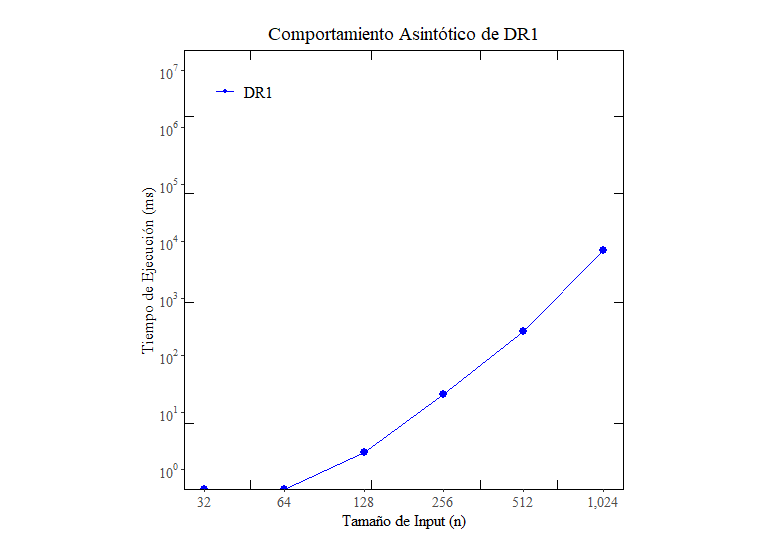
\includegraphics[width=15cm]{DR1_PLOT.png}}
  \end{center}

  Este algoritmo introduce el concepto de subdividir las matrices que se están multiplicando en matrices más pequeñas, para luego multiplicar las sub-matrices en lugar de aplicar una multiplicación bruta elemento por elemento, como lo hace el algoritmo tradicional. En el enunciado podemos ver lo siguiente, en donde \textit{A} y \text{B} son las matrices que se están multiplicando, y \textit{C} la matriz producto.

  \begin{center}
    $ C11 = A_{11} \cdot B_{11} + A_{12} \cdot B_{21} $\\
    $ C12 = A_{11} \cdot B_{12} + A_{12} \cdot B_{22}$\\
    $ C21 = A_{21} \cdot B_{11} + A_{22} \cdot B_{21} $\\
    $ C22 = A_{21} \cdot B_{12} + A_{22} \cdot B_{22} $\\
  \end{center}

  Sabemos que la suma de las matrices es de complejidad $O(n^2)$, por lo que la complejidad temporal puede escribirse como:

  \begin{center}
    $ T(n) = 8T(n/2) + O(n^2) $
  \end{center}

  Aplicando el \textbf{Teorema Maestro Simple}, en su tercera opción, obtenemos que:

  \begin{center}
    $ T(n) = O(n^{\log_28}) $ \\
    $ T(n) = O(n^3) $
  \end{center}

  La complejidad de DR1 es parecida a la del algoritmo tradicional, pero se debe tener en cuenta que esta es la expresión más básica del algoritmo de divide y conquista para este propósito.

  En segundo lugar, DR2 representa la implementación del algoritmo de Strassen, el cual lleva un paso más adelante la estrategia de divide y conquista. El algoritmo de Strassen también divide las matrices, pero éste elimina una de las llamadas recursivas, quedando únicamente en 7. Su comportamiento asintótico puede verse en el siguiente gráfico:

  \begin{center}
    \makebox[0pt]{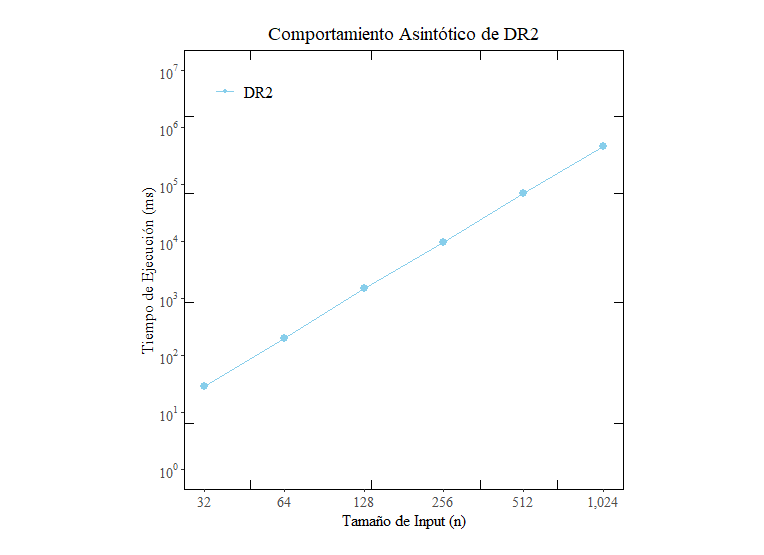
\includegraphics[width=15cm]{DR2_PLOT.png}}
  \end{center}

  En el enunciado podemos ver lo siguiente, en donde A y B son las matrices que se están multiplicando, y C la matriz producto.

  \begin{center}
    $ M = (A_{11} + A_{22})(B_{11} + B_{22}) $ \\
    $ N = (A_{21} + A_{22})B_{11} $ \\
    $ O = A_{11}(B_{12} - B_{22}) $ \\
    $ P = A_{22}(B_{21} - B_{11}) $ \\
    $ Q = (A_{11} + A_{12})B_{22} $ \\
    $ R = (A_{21} - A_{11})(B_{11} + B_{12}) $\\
    $ S = (A_{12} - A_{22})(B_{21} + B_{22}) $ \\
    $ C_{11} = M + P - Q + S $ \\
    $ C_{12} = O + Q $ \\
    $ C_{21} = N + P $ \\
    $ C_{22} = M + O - N + R $
  \end{center}

  La complejidad temporal de este algoritmo es entonces:

  \begin{center}
      $ T(n) = 7T(n/2) +  O(n^2) $
  \end{center}

  Por \textbf{Teorema Maestro Simple}, aplicando la opción 3, obtenemos:

  \begin{center}
    $ O(n^{Log7}) \approx O(n^{2.8074}) $
  \end{center}

  Por último, se muestra una vista comparativa entre DR1 y DR2, y una vista general de esos dos algoritmos junto con el algoritmo tradicional.

  \begin{center}
    \makebox[0pt]{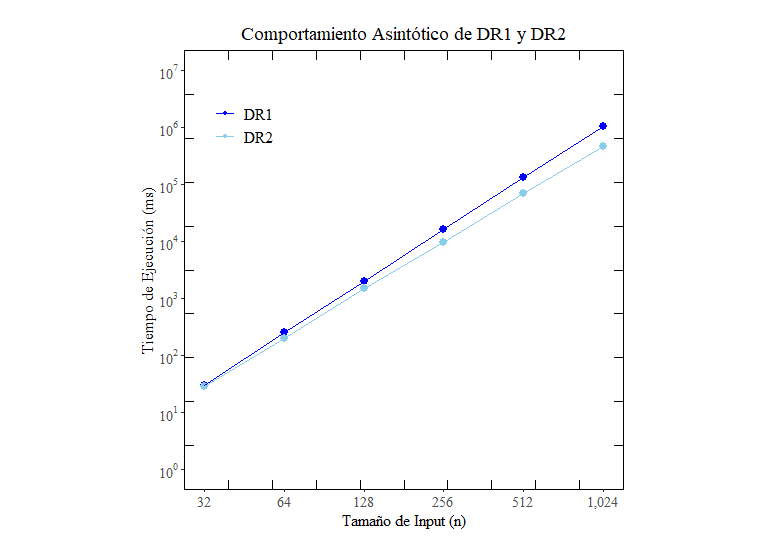
\includegraphics[width=15cm]{DR1_DR2_PLOT.png}}
  \end{center}

  \begin{center}
    \makebox[0pt]{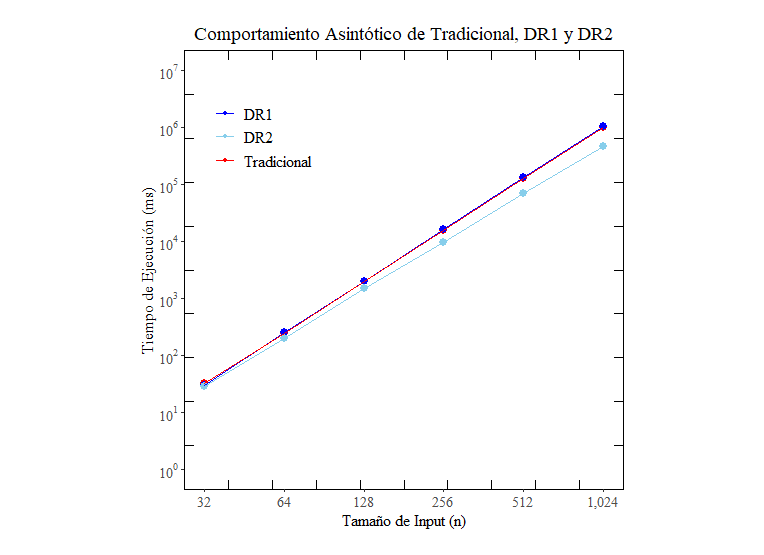
\includegraphics[width=15cm]{TRADITIONAL_DR1_DR2_PLOT.png}}
  \end{center}
\end{document}
